\documentclass[t]{beamer} % t = top alignment for frame content


%% IF YOU ARE MAKING ANY CHANGES, COMPILE TWICE! 
%% Tikz requires two compilations with pdf latex in order to get relative positioning information! 

\usepackage{etoolbox}
% Switch language (compile twice! -> babel package needs to be reloaded)
\newtoggle{lang_eng}
\settoggle{lang_eng}{false} % true: english, false: german (compile twice)


%% Include common useful packages
%% The following commented packages are included in the Beamer style template
%%\usepackage{pgfcomp-version-0-65}
%%\usepackage{xcolor}
%%\usepackage{graphicx}
%%\usepackage{pgfplots}
%%\usepackage{epstopdf}
%%\usepackage{changepage}
%%\usepackage{etoolbox}
%%\usepackage{helvet}


\usepackage[utf8]{inputenc}
\usepackage[\iftoggle{lang_eng}{english}{ngerman}]{babel}

\usepackage[justification=centering]{caption} % Justification: center captions by default
\captionsetup{textfont=scriptsize, font=scriptsize,labelfont=scriptsize}
\captionsetup[subfigure]{skip=7pt} % vertical spacing between figure and subfigure caption
\captionsetup{aboveskip=3pt} % vertical spacing between subfigure caption and figure caption (\baselineskip + aboveskip)
\captionsetup{belowskip=3pt} % vertical spacing between subfigure caption and figure caption (\baselineskip + aboveskip)

%% REMOVE LABELS a), b), ... Put this into figure environments for local settings
%\captionsetup[figure]{labelformat=empty}
%\captionsetup[subfigure]{labelformat=empty} 
%\captionsetup[table]{labelformat=empty}
%% You can easily hide labels by using \caption*{} instead of \caption{}

%\captionsetup[subfigure]{labelformat=empty}
%\setbeamerfont{caption}{size=\tiny}

\usepackage{hyperref}

\usepackage{listings} % Für Code

\usepackage[locale=DE]{siunitx} % Für Einheiten


\usepackage{mathtools,amssymb,amsmath}

\usepackage{pgfpages} % required for showing notes on the second screen

\usepackage{algorithm} % selber eingebunden
\usepackage[noend]{algpseudocode} % Alternative Algorithmenumgebung
\newcommand*\Let[2]{\State #1 $\gets$ #2}

\usepackage{booktabs}

\usepackage{subcaption}

% Textbox
\usepackage{grid-system}


\usepackage{ifplatform}






%% Include Videos
%% If you have compilation issues remove packages "l3kernel" and "l3packages" and reinstall them using miktex package manager.
%% Properly synchronize the package manager before.
%% Doc:  http://ftp.fau.de/ctan/macros/latex/contrib/media9/doc/media9.pdf
%% Example at the end of Zusammenfassung.tex (but commented out!)
%\usepackage{media9}

%% Enable Animations
%% You can easily create animations in combination with tikz,
%% Checkout the commented example in Zusammenfassung.tex and uncomment \usepackage{animate}
%\usepackage{animate}


%% Set title image
\newcommand{\titleImage}{TitelRobotik} % TitelRobotik, TitelAutomotive, TitelMechatronik, TitelEvoAlg, or custom image name!
\newcommand{\titleLocation}{Name der Veranstaltung, Ort, TT. - TT. Monat JJJJ}
\newcommand{\titleName}{Titel des Vortrages}
\newcommand{\titleAuthors}{\underline{Autor}, Koautoren}

\newcommand{\lastImageOtherOne}{TitelMechatronik}
\newcommand{\lastImageOtherTwo}{TitelAutomotive}


\newenvironment{wideitemize}{\itemize\addtolength{\itemsep}{10pt}}{\enditemize}
\newenvironment{bitemize}{\begin{itemize}[<+->]}{\end{itemize}} % This environment can be used to fade in items subsequently

\mode<presentation>
{
	\usetheme{RST}
	% How should covered items be treated (in bitemize environment or \pause)
	% Select transparent, invisible or only.
	% This setting can be overwritten by placing it before the specific code.
	\setbeamercovered{transparent = 28} % invisible, only
}
\setbeameroption{hide notes} % show/hide notes
\setbeamertemplate{note page}[plain]

%% Highlight text with \highlightGreen{} and \highlightOrange{}!

\begin{document}

% disable externalize by default
\externalizeOff
% Best practice is to enable externalization just for selected images using the environment
%\begin{externalize} \end{externalize} around the tikzpicture (this environment is defined in beamerthemeRST.sty) 



% Include content
\section{Einleitung}

% Für jede Folie eine Frame-Umgebung erstellen
% Innerhalb der Frame-Umgebung werden dann die Inhalte geschrieben

\begin{frame}
	\frametitle{Folientitel}
	
		\begin{itemize}
 			\item Dies ist ein Beispiel der ersten Ebene
 			\begin{itemize}
	 			\item Zweite Ebene mit \highlightGreen{hervorzuhebenden} Ausdruck
	 			\item Dies ist ein weiterer Stichpunkt in der zweiten Ebene
	 			\begin{itemize}
		 			\item Es gibt auch eine dritte Ebene, die selten zur Verwendung kommen sollte
	 			\end{itemize}
 			\end{itemize}
 			\item Zur Demonstration noch ein Stichpunkt in der ersten Ebene
 		\end{itemize}
 		
 		\begin{enumerate}
 		\item Es gibt auch \highlightOrange{Aufzählungen}
 		\item Diese Zeile sollte mit einer Zwei starten
 		\end{enumerate}
 		
\end{frame}



\begin{frame}
	\frametitle{Blöcke}
		\begin{itemize}
		 %\setlength\itemsep{1em} % CHANGE SPACING BETWEEN ITEMS
			\item Beispieltstichpunkt Ebene 1
			\item Und noch ein Beispielstichpunkt
		\end{itemize}
		
		\begin{block}{Dies ist ein Block}
 		      Mit normalem Text
 		      \begin{itemize}
 		        \item Und einer Aufzählung im Block.
 		        \item Ein weiterer Stichpunkt.
 		      \end{itemize}
		\end{block}
		
 		\begin{alertblock}{Dies ist ein anderer Block}
		   Mit normalem Text
		   \begin{itemize}
		     \item Und einer Aufzählung im Block.
		     \item Ein weiterer Stichpunkt.
		   \end{itemize}
 		\end{alertblock}
 		
\end{frame}

\begin{frame}[fragile]{Es geht weiter}
	 		\begin{exampleblock}{Falls die Farben nicht ausreichen: Ein weiterer Block}
				\setlength\abovedisplayskip{0pt} % remove spacing befor equations
				\begin{gather*}
				V^*(\mathcal{B}) = \underset{\mathcal{B}}{\min} \quad (n-1) \Delta T \label{eq:teb_olop} \\
				\begin{align*}
				\text{subject to} \\ 
				\quad & \mathbf{x}_1 = \mathbf{x}_s, \quad \mathbf{x}_n = \mathbf{x}_f , \quad \Delta T > 0 \hspace{-1cm}\\
				\quad & \mathbf{h}_k (\mathbf{x}_{k+1},\mathbf{x}_k,\mathbf{u}_k,\Delta T) = \mathbf{0} & (k=1,2,\dotsc,n-1)\\
				\quad & \mathbf{g}_1 (\mathbf{u}_1) \ge \mathbf{0} \\
				\quad & \mathbf{g}_k (\mathbf{x}_k,\mathbf{u}_k) \ge \mathbf{0} & (k=2,3,\dotsc,n-1)
				\end{align*}
				\end{gather*}
	 		\end{exampleblock}
\end{frame}


\begin{frame}{Keine Grenzen}
\tikzstyle{every picture}+=[remember picture]
\tikzstyle{na} = [baseline=-.5ex]	
\tikzstyle{background grid}=[draw, black!50,step=.5cm]
	
\vspace{\baselineskip}
	\begin{columns}[c] % center content
		\begin{column}{0.3\textwidth}
			\begin{itemize}
				\item Treibscheibe \tikz[na] \coordinate (item-tscheibe);
				\item Motor \tikz[na] \coordinate (item-motor);
				\item Gegengewicht \tikz[na] \coordinate (item-ggewicht);
				\item Lift \tikz[na] \coordinate (item-lift);
			\end{itemize}
		\end{column}
		\begin{column}{0.3\textwidth}
			% Use a background grid to make it easier to find coordinates
			% When the coordinates have been found, remove the 
			% 'show background grid' option. 
			\begin{tikzpicture}%[show background grid]
				\node [anchor = north west]{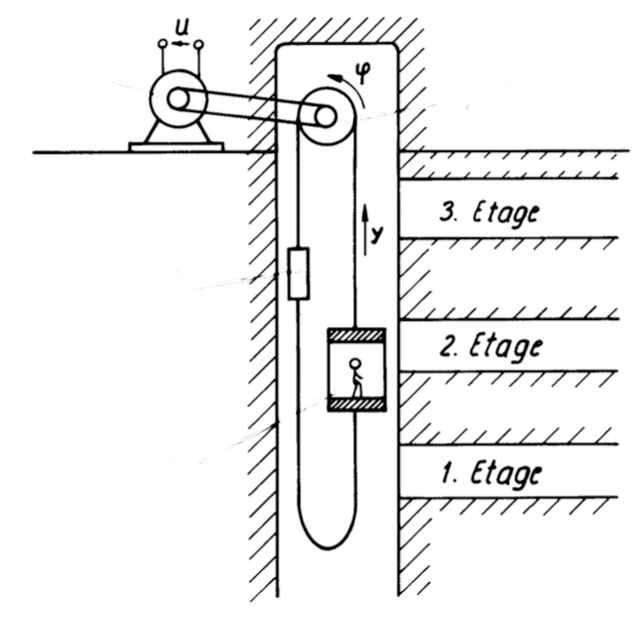
\includegraphics[width=3cm]{Aufzug.png}};
				%\fill (0,0) circle (2pt); % show origin
				% Destination coordinates
				\path (1.6, -0.5) coordinate (tscheibe)
						(0.6,-0.5) coordinate (motor)
						(1.2,-1.5) coordinate (ggewicht)
						(1.7,-2.1) coordinate (lift);
			\end{tikzpicture}
		\end{column}
	\end{columns}	

	% define overlays
	% Note the use of the overlay option. This is required when 
	% you want to access nodes in different pictures (in combination with remember picture).
	\begin{tikzpicture}[overlay]
		\path[->,RSTorange,thick] (item-tscheibe) edge [out=0, in=110] (tscheibe);
		\path[->,RSTgreen,thick] (item-motor) edge [out=0, in = 180] (motor);
		\path[->,RSTblue,thick] (item-ggewicht) edge [out=0, in = -170] (ggewicht);
		\path[->,RSTyellow,thick] (item-lift) edge [bend right] (lift);
	\end{tikzpicture}

\end{frame}


\section{Modellbildung}


% Für jede Folie eine Frame-Umgebung erstellen
% Innerhalb der Frame-Umgebung werden dann die Inhalte geschrieben


\begin{frame}[fragile]
	\frametitle{Bild neben Bild}
		\begin{itemize}
			\item Beispieltstichpunkt Ebene 1
			\item Und noch ein Beispielstichpunkt
 		\end{itemize}

\begin{figure}[htbp]
        \centering

        \begin{subfigure}[b]{0.45\textwidth}
        		\centering
                
\includegraphics[width=\textwidth]{mechatronisches_antriebsystem.png} % relative width w.r.t. to the subfigure box
                \caption*{Struktur eines Antriebsystems}  % Hide label using \caption*{} instead of \caption
                \label{fig:myfigure2a}
        \end{subfigure}%
        \quad %add desired spacing between images, e. g. ~, \quad, \qquad, \hfill etc.
          %(or a blank line to force the subfigure onto a new line)
        \begin{subfigure}[b]{0.45\textwidth}
        		\centering
        		              
        		% You may insert \includegraphics here, but this is an example for tikz images:
        		\begin{externalize}
                \begin{tikzpicture}[align=center,auto]
	                % Tikz example adapted from http://www.texample.net/tikz/examples/tag/block-diagrams/
	                % Elemente
	                \tikzstyle{block} = [draw, rectangle, minimum height=1em, minimum width=2em]
	                \tikzstyle{sum} = [draw, circle]
	                \tikzstyle{every node}=[font=\tiny] % set fontsize for all nodes
	                
	                % Blöcke:
	                \node[coordinate] (input) {};
	                \node[sum] (sum) [right=0.4cm of input] {};
	                \node[block] (controller) [right=0.5cm of sum] {Controller};
	                \node[block] (system) [right=0.5cm of controller] {System};
	                \node[coordinate] (output) [right=0.6cm of system] {};
	                
	                % Verbindungen
	                \draw [->] (controller) -- node[name=u] {$u$} (system);
	                \draw [draw,->] (input) -- node {$w$} (sum);
	                \draw [->] (sum) -- node {$e$} (controller);
	                \draw [->] (system) -- node [name=y] {$y$}(output);
	                \draw [->] (y) |- ([yshift=-1em]system.south) -| node[pos=0.99] {$-$} node [near end] {$y_m$} (sum); %
                \end{tikzpicture}
                \end{externalize}
                \caption*{Allgemeine Reglerstruktur} % Hide label using \caption*{} instead of \caption
                \label{fig:myfigure2b}
        \end{subfigure}
        %\caption*{Blockschaltbilder}
        \label{fig:myfigure2}

	\begin{itemize}
		\item In den Abbildungen sieht man noch einmal den Unterschied zwischen Bitmaps (links) und Vektorgrafiken (rechts)
	\end{itemize}
\end{figure} 		
 		
\end{frame}



\begin{frame}{Zwei-Spalten Umgebung}


\begin{columns} % optional [c] or [T]
	\begin{column}{0.5\textwidth}
		Erste Spalte: 
		\begin{itemize}
			\item Nummer eins.
			\item Nummer zwei.
		\end{itemize}
	\end{column}
	\begin{column}{0.45\textwidth}
		Zweite Spalte:
		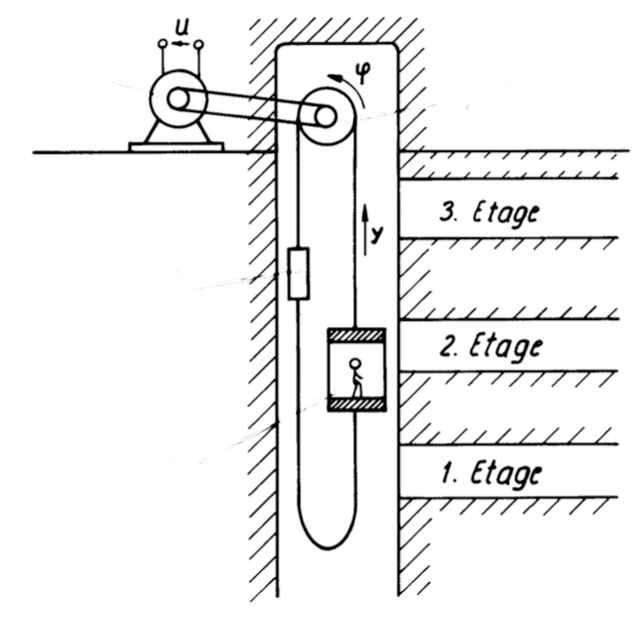
\includegraphics[width=0.9\columnwidth]{Aufzug.png}
	\end{column}
\end{columns}


\end{frame}


\section{Ergebnisse}


% Für jede Folie eine Frame-Umgebung erstellen
% Innerhalb der Frame-Umgebung werden dann die Inhalte geschrieben

\begin{frame}
	\frametitle{Platzhalter}
		\begin{itemize}
			\item Beispieltstichpunkt Ebene 1
			\item Und noch ein Beispielstichpunkt
 		\end{itemize}
 		
 		\begin{center}
 		\begin{tikzpicture}[->,>=stealth',shorten >=1pt,auto,node distance=3cm, thick]
 		  \tikzstyle{main node}=[circle,fill=RSTgreen!50,draw,font=\sffamily\Large\bfseries]
 		  \node[main node] (1) {1};
 		  \node[main node] (2) [below left of=1] {2};
 		  \node[main node] (3) [below right of=2] {3};
 		  \node[main node] (4) [below right of=1] {4};
 		
 		  \path[every node/.style={font=\sffamily\small}]
 		    (1) edge node [left] {0.6} (4)
 		        edge [bend right] node[left] {0.3} (2)
 		        edge [loop above] node {0.1} (1)
 		    (2) edge node [right] {0.4} (1)
 		        edge node {0.3} (4)
 		        edge [loop left] node {0.4} (2)
 		        edge [bend right] node[left] {0.1} (3)
 		    (3) edge node [right] {0.8} (2)
 		        edge [bend right] node[right] {0.2} (4)
 		    (4) edge node [left] {0.2} (3)
 		        edge [loop right] node {0.6} (4)
 		        edge [bend right] node[right] {0.2} (1);
 		\end{tikzpicture}
 		\end{center}

 		
\end{frame}


\begin{frame}{Tikz Plotting}

\begin{figure}[htb]
	\centering	
	\begin{tikzpicture}%[trim axis left]
		\begin{axis}[
		  width = 0.9\textwidth,
		  height = 4cm,
		  domain = 0.001:10,
		  samples = 100,
		  grid = both,
		  xlabel = $\delta$,
		  ylabel = Weights,
		  legend pos = south east] % customize the axis environment with whatever you want (xmax,ymin,...)	  
		\addplot [color=black, solid, line width=1.5pt] {0.5*tanh(x-3)+0.5}; \addlegendentry{$\sigma$};
		\addplot [color=gray, dashed, line width=1.5pt] {1-(0.5*tanh(x-3)+0.5)}; \addlegendentry{$(1-\sigma)$};
		\end{axis}
	\end{tikzpicture}
	\caption{Plot with Tikz (without any Matlab export)}
\end{figure}

\end{frame}

\begin{frame}{Itemsep}

\begin{itemize}
	\setlength{\itemsep}{\baselineskip}
	\item If you only have a few items on the slide
	\item you might increase the item separation
	\item just insert \texttt{\textbackslash setlength\{\textbackslash itemsep\}\{\textbackslash baselineskip\}} into the \texttt{itemize} environment.
	\item Some small adjustments between multiple environments (figure, table, itemize) can be adjusted by simply inserting \texttt{\textbackslash vspace\{positive or negative value\}}.
	\item \texttt{\textbackslash vspace\{$\pm$\textbackslash baselineskip\}} removes or adds a complete line.
	\item If you have a lot of spacing in the beginning of a block, try \texttt{\textbackslash fixSpacing} at the beginning of the block.
\end{itemize}

\end{frame}

\section{Zusammenfassung}


% Für jede Folie eine Frame-Umgebung erstellen
% Innerhalb der Frame-Umgebung werden dann die Inhalte geschrieben


\begin{frame}
	\frametitle{Platzhalter}

	% Define block styles
	\tikzstyle{decision} = [diamond, draw, fill=RSTgreen!50, 
	    text width=4.0em, text badly centered, node distance=2cm, inner sep=0pt]
	\tikzstyle{block} = [rectangle, draw, fill=RSTgreen!50, 
	    text width=5em, text centered, rounded corners, minimum height=2em]
	\tikzstyle{line} = [draw, -latex']
	\tikzstyle{cloud} = [draw, ellipse,fill=RSTorange!60, node distance=3cm, minimum height=2em]
	    
	\begin{center}
	\begin{tikzpicture}[node distance = 1.4cm, auto, every node/.style={font=\sffamily\scriptsize}]
	    % Place nodes
	    \node [block] (init) {initialize model};
	    \node [cloud, left of=init] (expert) {expert};
	    \node [cloud, right of=init] (system) {system};
	    \node [block, below of=init] (identify) {identify candidate models};
	    \node [block, below of=identify] (evaluate) {evaluate candidate models};
	    \node [block, left of=evaluate, node distance=3cm] (update) {update model};
	    \node [decision, below of=evaluate] (decide) {is best candidate better?};
	    \node [block, below of=decide, node distance=1.9cm] (stop) {stop};
	    % Draw edges
	    \path [line] (init) -- (identify);
	    \path [line] (identify) -- (evaluate);
	    \path [line] (evaluate) -- (decide);
	    \path [line] (decide) -| node [near start] {yes} (update);
	    \path [line] (update) |- (identify);
	    \path [line] (decide) -- node {no}(stop);
	    \path [line,dashed] (expert) -- (init);
	    \path [line,dashed] (system) -- (init);
	    \path [line,dashed] (system) |- (evaluate);
	\end{tikzpicture}
	\end{center}
 		 		
\end{frame}

\begin{frame}{Weitere Beispiele}
	\setbeamercovered{transparent} % invisible / transparent
	\begin{bitemize}
		\item Dies ist das erste Item.
		\item Dies ist das zweite Item.
		\item Dies ist das dritte Item.
	\end{bitemize}
	
	\setbeamercovered{invisible}
	\pause
	Es gibt auch einen Pausebefehl!

\end{frame}

%\begin{frame}{Tikz animation example}
%	\begin{center}
%	\begin{animateinline}[controls=false,autoplay,palindrome,loop]{10}
%		\multiframe{50}{nYinc=-0.5+0.02, nAngleA=0+0.5, nAngleB=-180+0.5, nColor=0+2}{
%		\makebox[0.8\textwidth]{
%			\begin{tikzpicture}
%				\tikzstyle{circlestyle}=[gray];
%				\tikzstyle{trajectory}=[shorten <= 0.1cm, shorten >= 0.1cm];
%				\node [rectangle, minimum width= 5cm, minimum height = 3cm, anchor = center] at (0,0) {};
%				\filldraw[circlestyle] (-3,0) circle (0.1cm) coordinate (start) node[above] {\small Start};
%				\filldraw[circlestyle] (3,0) circle (0.1cm) coordinate (goal) node[above] {\small Goal};
%				\node[anchor = south] (top) at (0, 0.5) {\small $\tau_1$};
%				\coordinate (middle) at (0,\nYinc);
%				\node[anchor = south] (bottom) at (0,-0.5) {\small $\tau_2$};
%				\draw[trajectory, line width=0.5mm, color=RSTgreen] (start) to[out=0, in=-155]  (top.south) to[out=25, in=180] (goal);
%				\draw[trajectory, line width=0.4mm, color=RSTgreen!\nColor!RSTorange] (start) to[out=0, in=\nAngleB] (middle) to[out=\nAngleA, in=180] (goal);
%				\draw[trajectory, line width=0.5mm, color=RSTorange] (start) to[out=0, in=180] (bottom.south) to[out=0, in=180] (goal);]
%			\end{tikzpicture}
%			}
%		}
%	\end{animateinline}
%	\end{center}
%\end{frame}

%\begin{frame}[fragile]{Video}
%
%	\begin{center}
%		\includemedia[
%			width=0.6\linewidth,keepaspectratio,
%			addresource=Videos/FILENAME.mp4,
%			transparent, %transparent player background
%			activate=onclick, % pageopen or onclick
%			passcontext, %show VPlayer’s right-click menu
%			flashvars={
%				source=VIDEO_PATH
%				&loop=true % loop video
%				&autoPlay=true
%			}
%		]{\includegraphics{PREVIEW_IMAGE_PATH}}{VPlayer.swf}
%	\end{center}
%
%   BUT ITS'S SMARTER TO USE OUR FANCY MACRO:
%%	\begin{center}
%%		\placeVideo[onclick]{VIDEO_PATH}{PREVIEW_IMAGE_PATH}{0.6\linewidth} % onclick or pageopen
%%	\end{center}
%%  This macro is able to detect, if the package media9 was loaded properly, otherwise only the preview image will be displayed.
%
%
%\end{frame}


% Generate final page
\generateFinalPage

% You might add backup slides here ...



\end{document}